\documentclass[../main.tex]{subfiles}

\begin{document}
Ovde je, na slici \ref{fig:paketi_teretane}, prikazana sekcija koja sadrži aktuelne pakete usluga koje ovaj sistem teretana pruža (dečije i PS). Ovo je jedna od sekcija kojoj može pristupiti samo registrovan i prijavljen korisnik (odnosno, klijent). Klijent bira paket o kome želi da dobije dodatne informacije klikom na vezu ``Prikaži više...``, koja vodi ka posebnoj stranici sa detaljnim opisom izabranog paketa i cenom. Ukoliko klijent, nakon usvajanja ovih informacija, i dalje želi taj paket, klikom na dugme ``Kupi paket`` započinje kupovinu. Naredni korak podrazumeva popunjavanje formulara, koji se prikazuje korisniku nakon sto je kliknuo na pomenuto dugme. U formularu navodi svoje osnovne informacije i bira program. Nakon što klijent pristane da nastavi dalje, prelazi se na formular za plaćanje, koji je detaljnije opisan u sekciji-------------------.

\begin{figure}[!ht]
\begin{center}
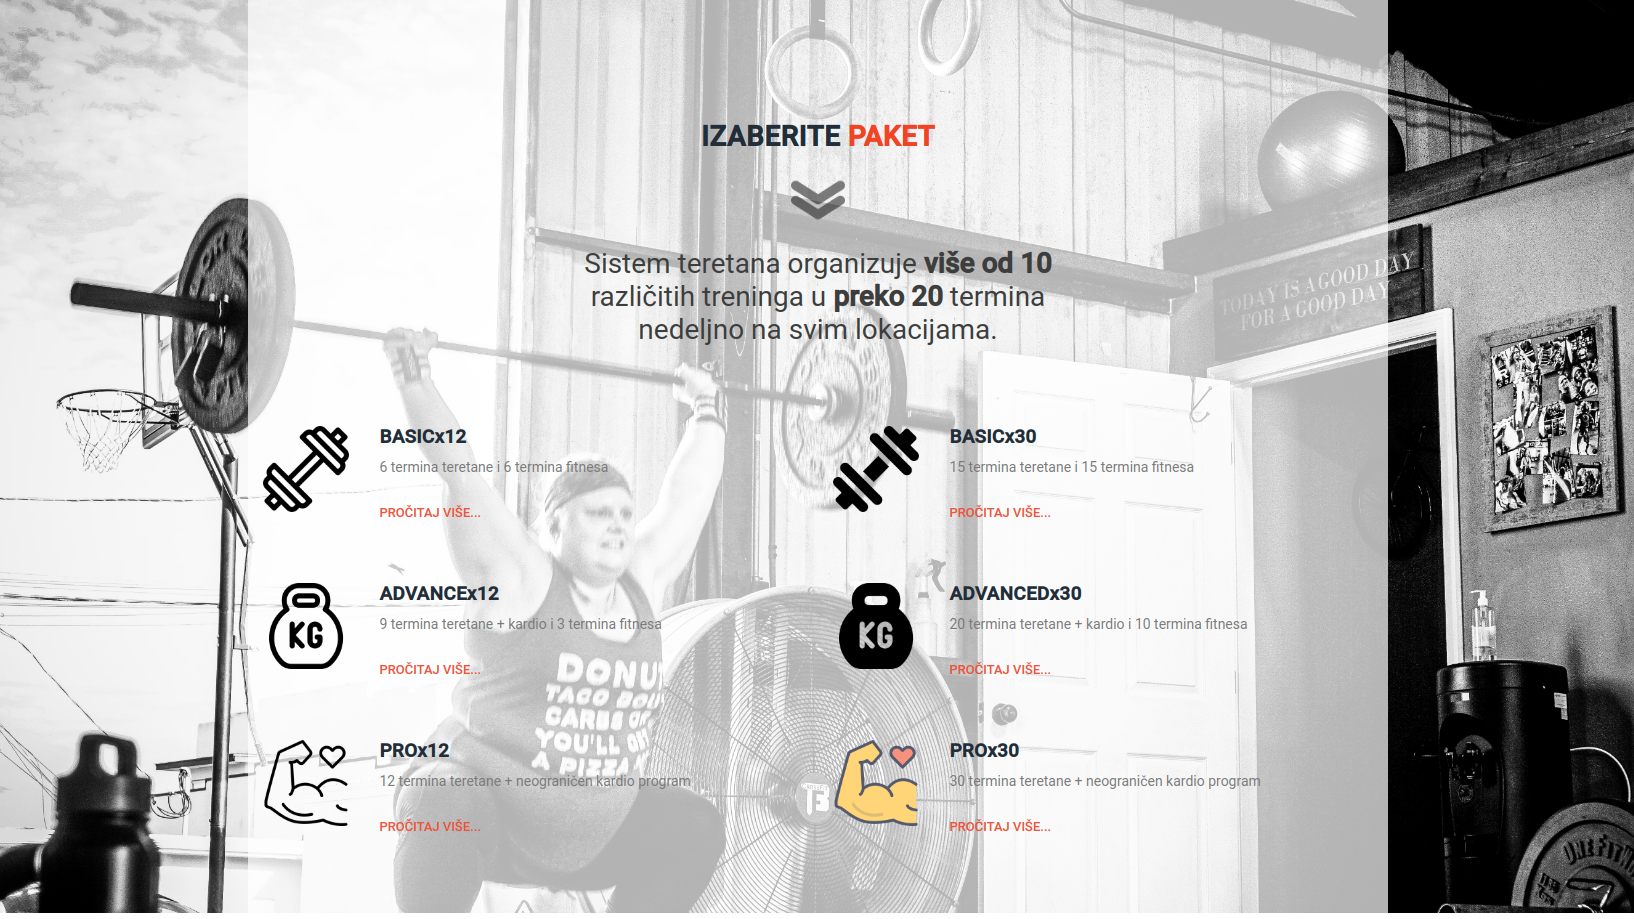
\includegraphics[scale=0.21]{sections/korisnicki_interfejs/screenshots/paketi_teretane.png}
\end{center}
\caption{Paketi usluga teretane}
\label{fig:paketi_teretane}
\end{figure}

U nastavku je prikazan izgled stranica koje sadrže opise paketa i cene. Na slici (\ref{fig:paketi} gore levo) je prikazana stranica u kojoj je dat opis paketa ``BASICx12``, na slici (\ref{fig:paketi} sredina levo) stranica u kojoj je dat opis paketa ``ADVANCEDx12``, dok je na slici (\ref{fig:paketi} dole levo) prikazana stranica sa opisom paketa ``PROx12``. Slede slike sa desne strane  \ref{fig:paketi}, na kojima su prikazane stranice u kojima su opisani paketi ``BASICx30``, ``ADVANCEDx30`` i ``PROx30`` redom.

\begin{figure}[!ht]
\begin{center}
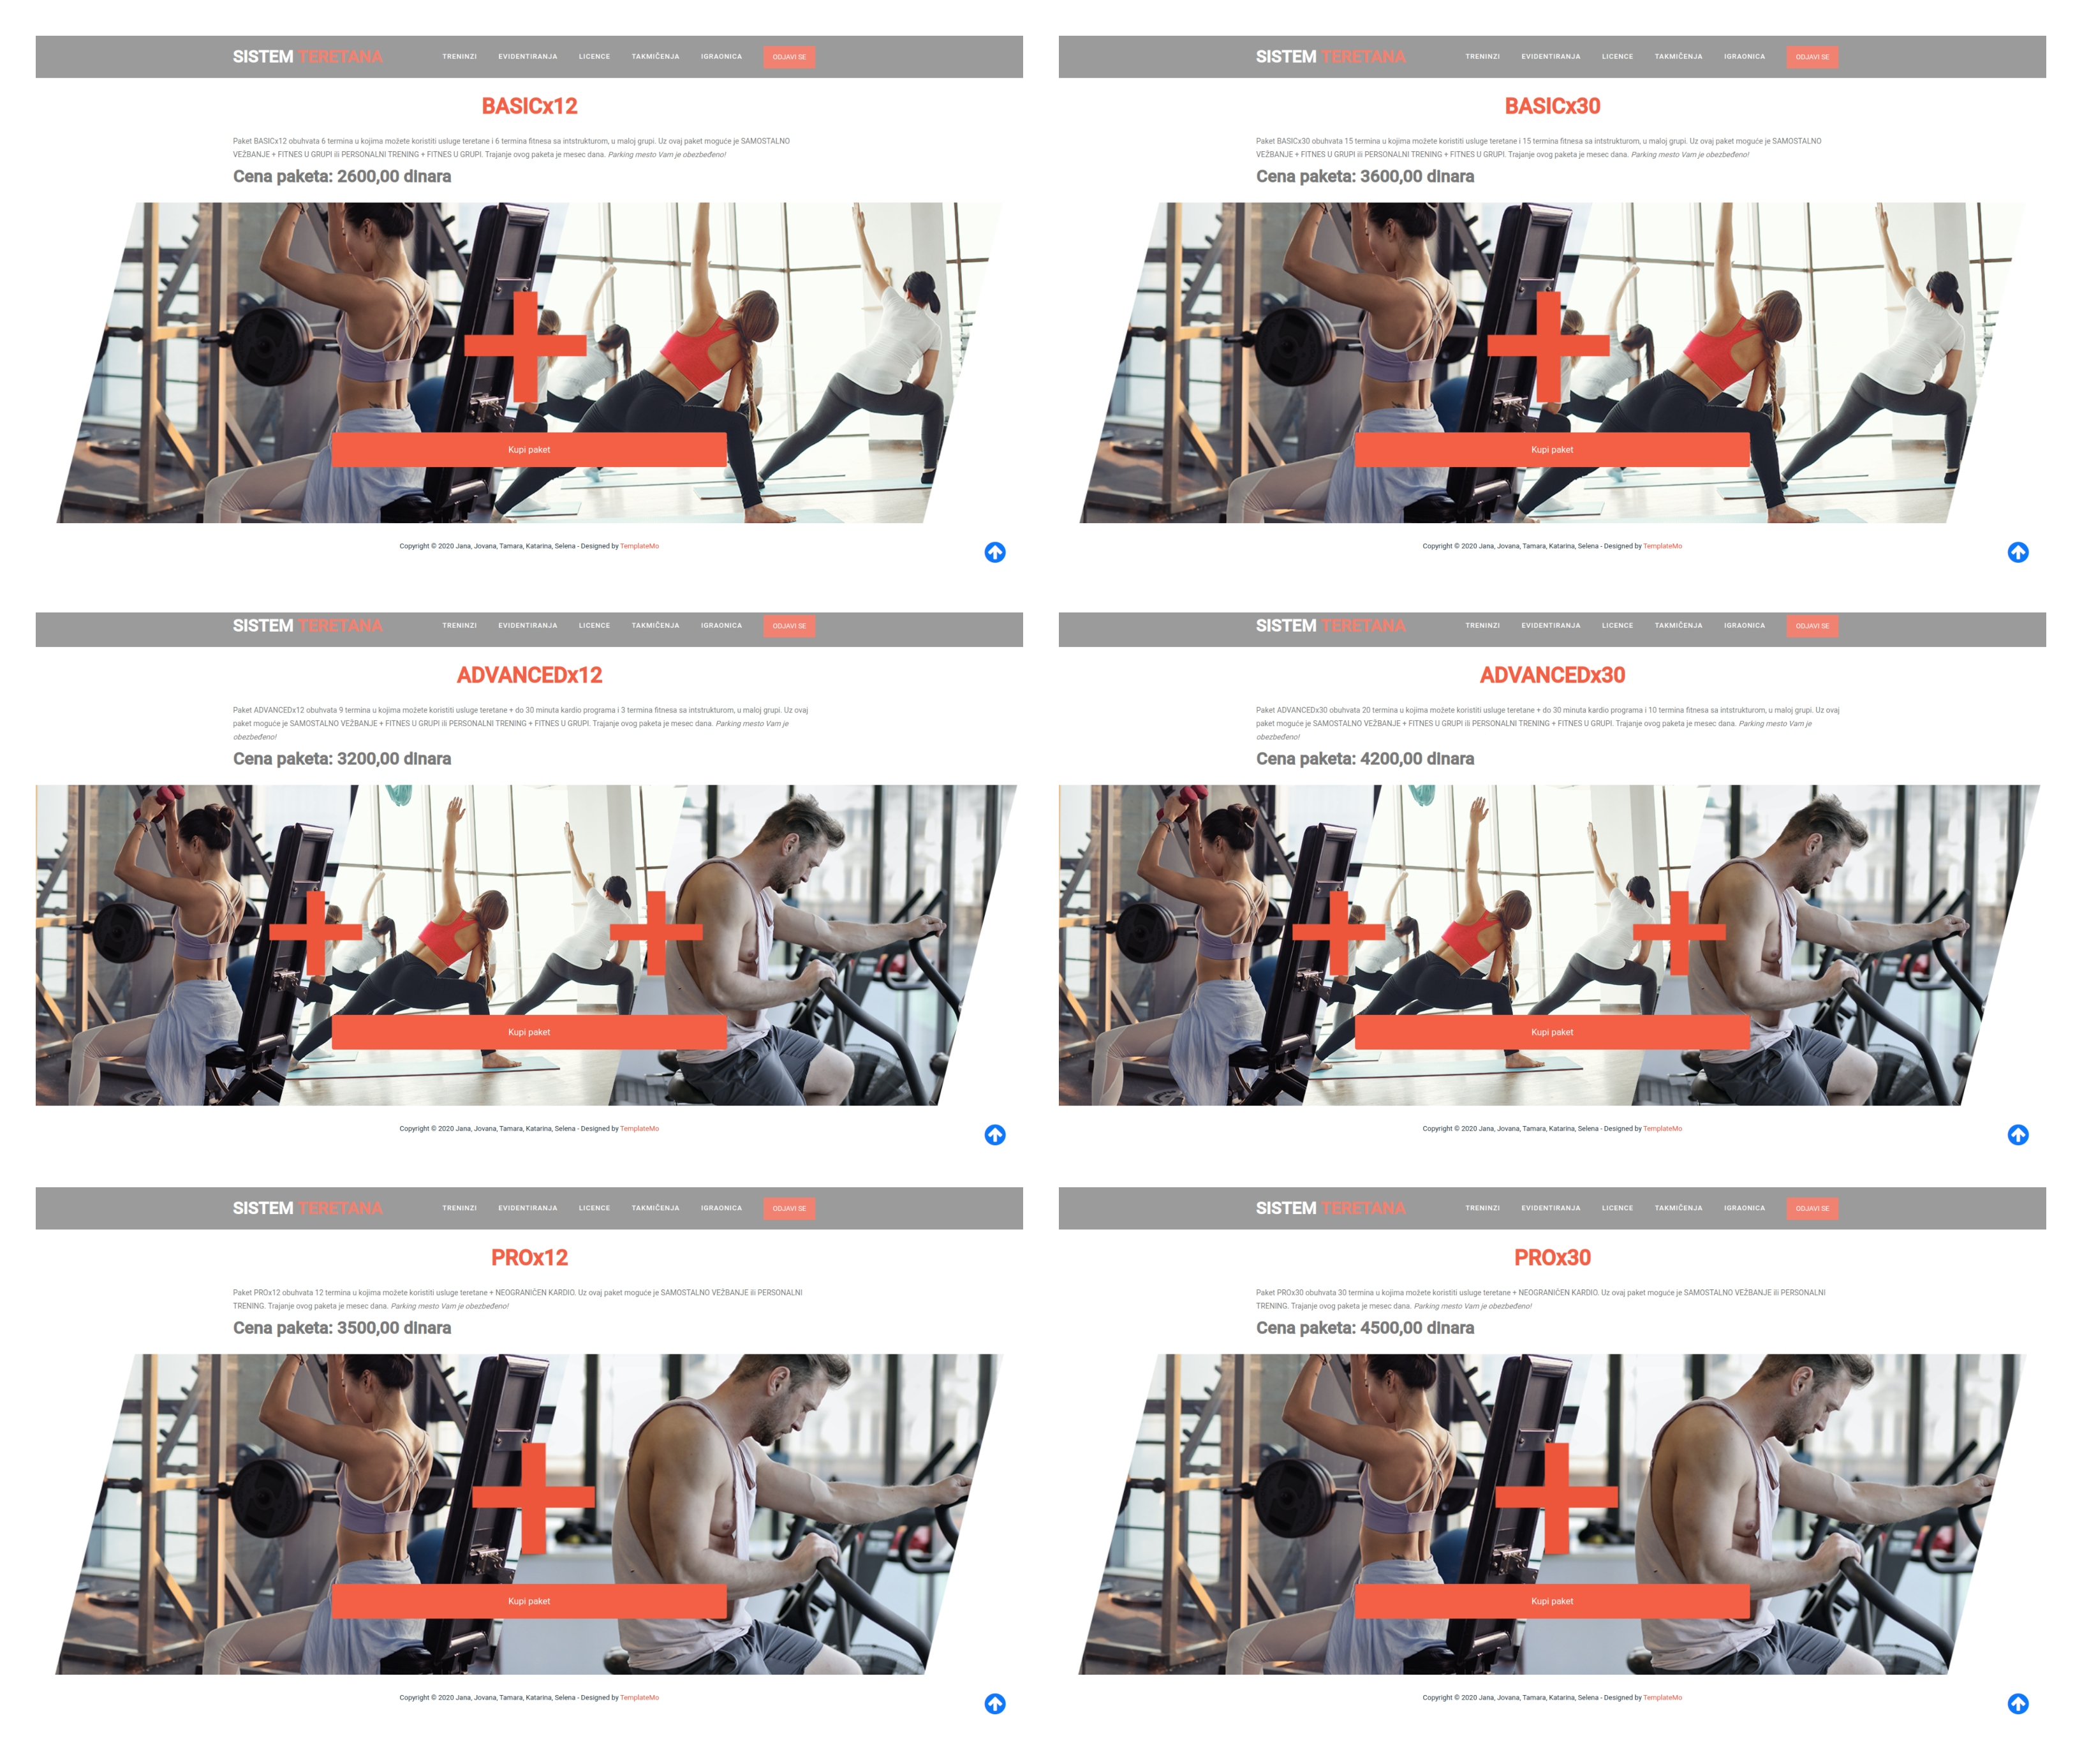
\includegraphics[scale=0.20]{sections/korisnicki_interfejs/screenshots/programiPaketi.jpg}
\end{center}
\caption{Gore levo:Opis paketa ``BASICx12``, Sredina levo: Opis paketa ``ADVANCEDx12``, Dole levo: Opis paketa ``PROx12``, Gore desno: Opis paketa ``BASICx30``, Sredina desno: Opis paketa ``ADVANCEDx30``, Dole desno: Opis paketa ``PROx30``}
\label{fig:paketi}
\end{figure}

\end{document}